\input{"tex/preamble"}

\graphicspath{ {./figures/} }

\hypersetup{
    colorlinks=true,
    linkcolor=black,
    urlcolor=cyan
}

\renewcommand*\contentsname{}

\begin{document}

\title{drylabproposal}
\author{iGEM UofT}
\date{}

%\maketitle

\begin{center}
    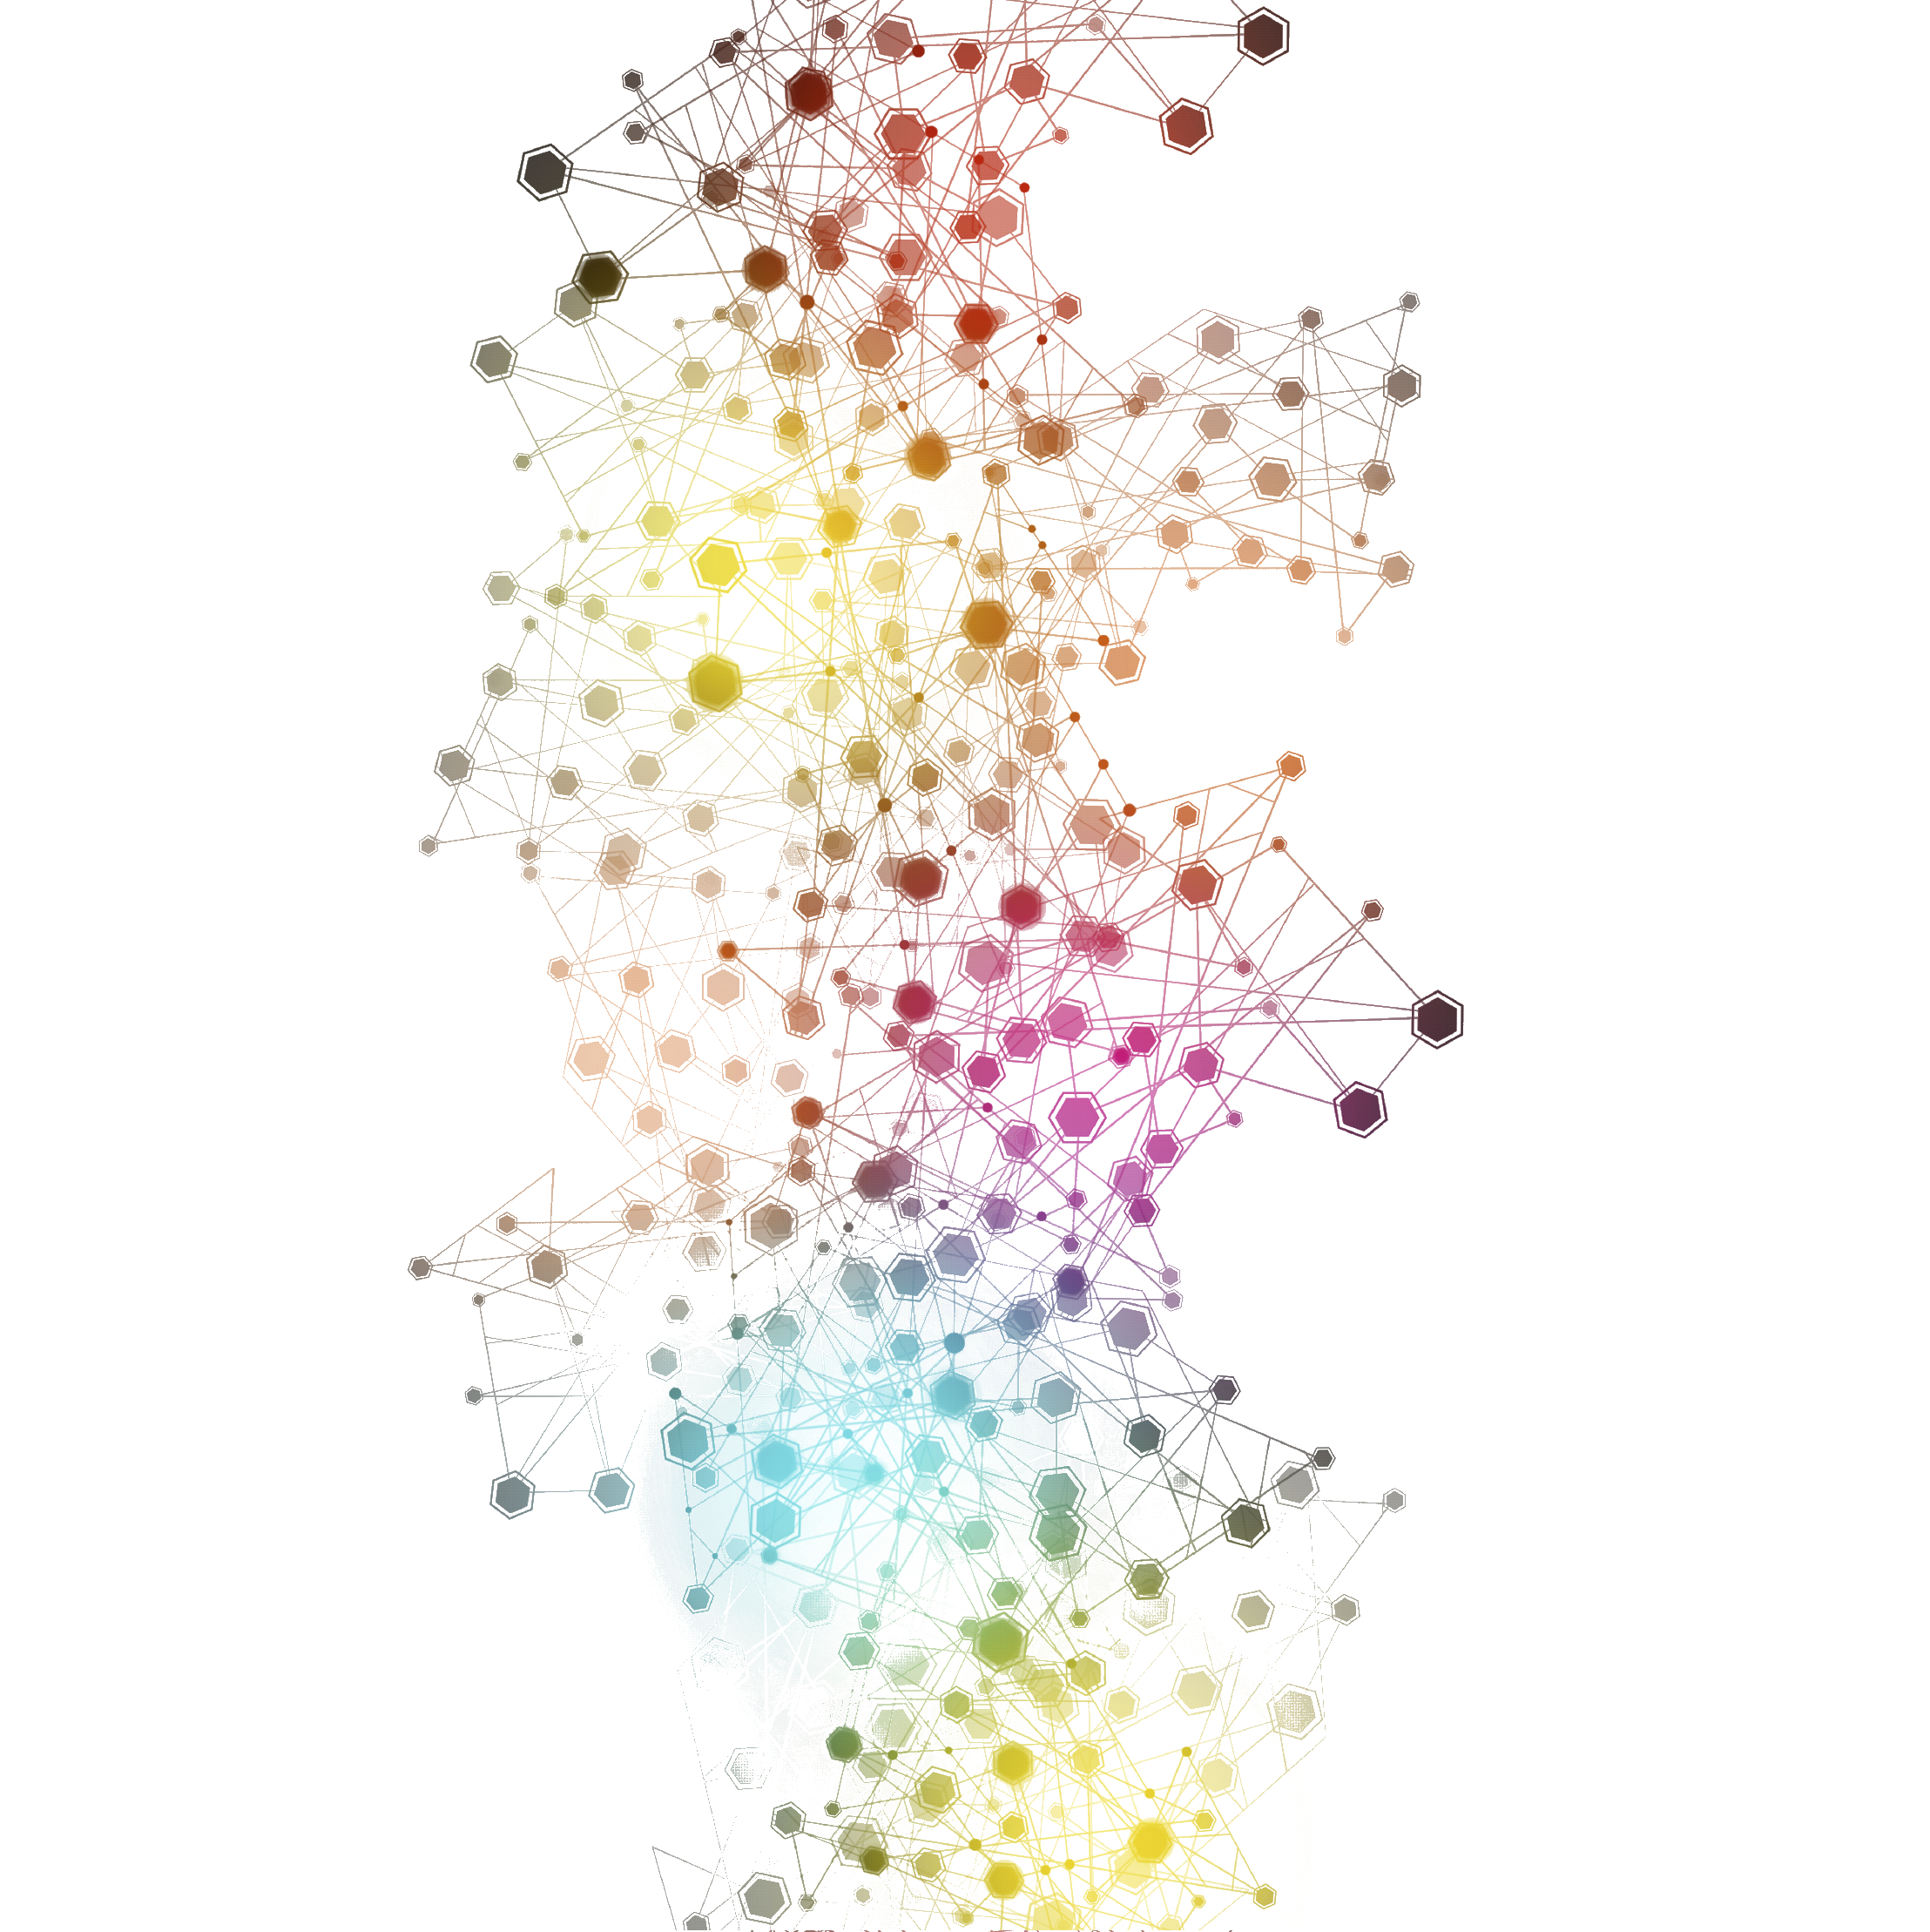
\includegraphics[width=0.9\textwidth]{global_transparent} \\
    \vspace{10pt}
    {\huge \textbf{\textit{2015 Dry Lab Proposal}}} \\
    \vspace{10pt}
    \includegraphics[width=0.2\textwidth]{igem_uoft} 
\end{center}

\tableofcontents

\thispagestyle{empty}

\newpage
\setcounter{page}{1}

\section{Abstract}

With the advancement of high throughput sequencing and large-scale proteomic
experiments, studying biology computationally and systematically has become
extremely useful and even necessary. Rapid advances in network biology has
elucidated many pathways and mechanisms important for many applications such as
drug development, disease prediction and biological engineering \cite{dry01}. We
propose to create a genetic circuit editor which uses iGEM's Registry of
Standard Biological Parts database \cite{dry02}. This editor will allow the user
to intuitively create genetic circuits from any part(s) listed in the registry
for any species that exists in our curated database. As a genetic circuit is
being built, our tool will also dynamically render a metabolic network
representing the metabolome of the species being worked on. Their metabolic
network will change dynamically as new parts are added to the circuit through
the addition of new nodes, new links, deletion of nodes, deletion of links and
changes in flux. Dynamic flux balance analysis will power all metabolic network
simulations \cite{dry03}. Lastly, our tool will allow the user to test their
engineered species in a microbiome setting by integrating the species's
metabolic network with the metabolic network of a user defined microbial
community.

\section{Methods}

Our tool will be built on a web-interface which uses MongoDB as its database.
User interface and graph rendering will be powered by the open source JavaScript
library d3.js. We will develop a pipeline for curating data and for creating our
database. Our pipeline will start with taking a ``point-in-time'' dump of the
2010 Registry of Standard Biological Parts database from iGEM's website as an
XML file. Using Python, we will parse through the  XML file and build our
MongoDB database of the registry. We will manually download proteomes from
public databases such as KEGG and Ensembl as .fasta files. Using the gene
annotations of all species, we will subsequently draft a dataset of all
interactions and reactions by using databases such as KEGG, Biocyc and Metacyc.
We will then manually validate each reaction and will correct false reactions
through manual curation. All gene interaction and reaction data will be stored
in our MongoDB database. By constructing stoichiometric matrices from a set of
user defined species, our tool will use flux balance analysis to simulate their
metabolome.

\section{Web Architecture}

\begin{center}
\resizebox{!}{0.95\textheight}{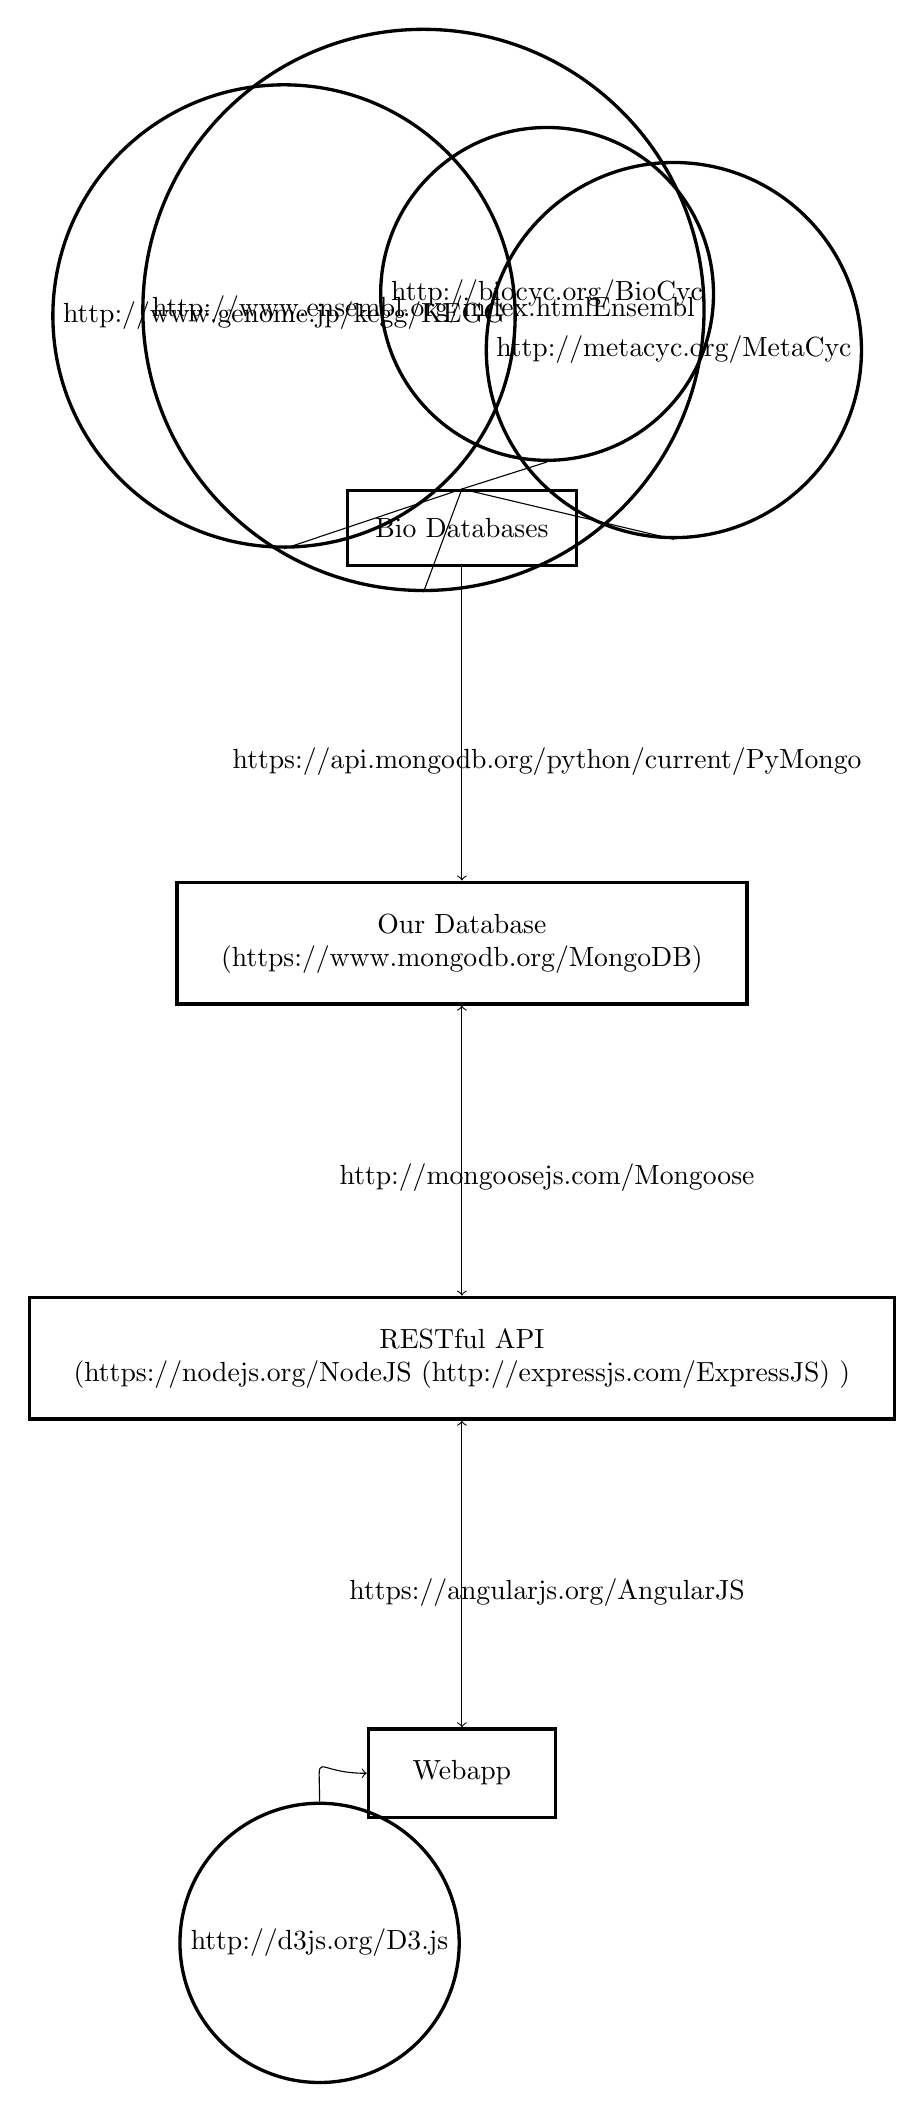
\begin{tikzpicture}[
    squarednode/.style={rectangle, draw=black, very thick, minimum size=5mm, inner sep=10pt},
    roundnode/.style={circle, draw=black, very thick, minimum size=7mm},
]

\node[squarednode] (biodatabases) {Bio Databases};

\path (biodatabases) ++(270:150pt) node[squarednode] (MongoDB) {\begin{tabular}{c} 
    Our Database \\
    (\href{https://www.mongodb.org/}{MongoDB})
\end{tabular}};

\path (biodatabases) ++(130:100pt) node [roundnode] (KEGG) {\href{http://www.genome.jp/kegg/}{KEGG}};
\path (biodatabases) ++(100:80pt) node [roundnode] (Ensembl) {\href{http://www.ensembl.org/index.html}{Ensembl}};
\path (biodatabases) ++(70:90pt) node [roundnode] (BioCyc) {\href{http://biocyc.org/}{BioCyc}};
\path (biodatabases) ++(40:100pt) node [roundnode] (MetaCyc) {\href{http://metacyc.org/}{MetaCyc}};

\path (biodatabases) ++(290:90pt) node[] {\href{https://api.mongodb.org/python/current/}{PyMongo}};

\path (MongoDB) ++(270:150pt) node [squarednode] (API) {\begin{tabular}{c}
    RESTful API \\
    (\href{https://nodejs.org/}{NodeJS} (\href{http://expressjs.com/}{ExpressJS}) )
\end{tabular}};

\path (API) ++(290:90pt) node[] (AngularJS) {\href{https://angularjs.org/}{AngularJS}};

\path (MongoDB) ++(290:90pt) node[] (Mongoose) {\href{http://mongoosejs.com/}{Mongoose}};

\path (API) ++(270:150pt) node [squarednode] (webapp) {\begin{tabular}{c}
    Webapp \\ 
\end{tabular}};

\path (webapp) ++(230:80pt) node [roundnode] (D3) {\href{http://d3js.org/}{D3.js}};


%\draw[->] (KEGG.south) .. controls +(down:7mm) and +(left:7mm) .. (biodatabases.west);
\draw[-] (KEGG.south) -- (biodatabases.north);
%\draw[->] (Ensembl.north) .. controls +(up:37mm) and +(left:55mm) .. (biodatabases.west);
\draw[-] (Ensembl.south) -- (biodatabases.north);
\draw[-] (BioCyc.south) -- (biodatabases.north);
\draw[-] (MetaCyc.south) -- (biodatabases.north);
\draw[->] (biodatabases.south) -- (MongoDB.north);
\draw[<->] (MongoDB.south) -- (API.north); 
\draw[<->] (API.south) -- (webapp);
\draw[->] (D3.north) .. controls +(up:7mm) and +(left:7mm) .. (webapp.west);

\end{tikzpicture}
}
\end{center}

\begin{thebibliography}{99\kern\bibindent}
\makeatletter
\let\old@biblabel\@biblabel
\def\@biblabel#1{\old@biblabel{#1}\kern\bibindent}
\let\old@bibitem\bibitem
\def\bibitem#1{\old@bibitem{#1}\leavevmode\kern-\bibindent}
\makeatother

\bibitem{dry01}
        http://www.nature.com/nbt/journal/v28/n12/full/nbt.1711.html
        
\bibitem{dry02}
	http://parts.igem.org/Registry\_API

\bibitem{dry03}
	http://www.ncbi.nlm.nih.gov/pmc/articles/PMC1302231/ 
\end{thebibliography}


\end{document}
